General relativity is a generalization of special relativity to include gravity. It has lead to many important discoveries,
as well as the whole field of cosmology. It is also one of the two main advancements of the 20th century, the second being, of course,
quantum mechanics. It is therefore important to understand at least the very basics of general relativity.
Note that this description is not completely rigorous, and tries to get the point across intuitively as well as mathematically.
Also worth pointing out is that you will need to understand the math explained in part one, especially the calculus. It will be very
hard to understand the rough derivation if you do not.
\section{Principle of Equivalence}
One of the first big things Einstein did was look at the following situation. Imagine you are in a box with no windows, on Earth, being pulled down
by gravity (or a force $g$). Now, imagine you are in a rocket, also with no windows, in outer space, accelerating with that same force $g$. 
\begin{figure}[H]
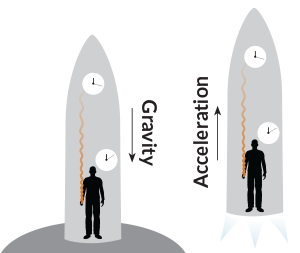
\includegraphics[scale=0.5]{equiv.png}
\end{figure}
Einstein said that there is no experiment that you could do to distinguish these situations. Try to come up with an experiment that you
think would distinguish the two. Why might it be wrong? I guarantee, however, that it is incorrect. 
So, these two situations are sort of the same - there's a fundamental equivalence between the two.
Now, let's imagine we are in that rocket again.
\begin{figure}[H]
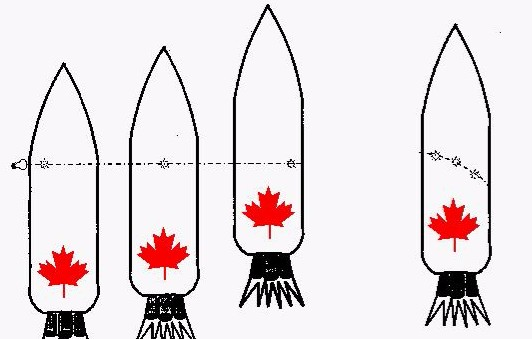
\includegraphics[scale=0.5]{relgen3.jpg}
\end{figure}
Imagine shining a flashlight from one side of the rocket to the other. From the point of view of an observer on the Earth,
the light goes in a straight line, but since the rocket is accelerating, the light appears to bend down from the point of view of
the observer in the rocket. Because the light is bending here, and we established that there is a fundamental equivalence between
this situation and that box on the Earth, the same thing must happen there, and it does. But we can draw a more general conclusion
from this: namely, that light bends in a gravitational field. This explained something interesting that had happened. In a solar
eclipse earlier, astronomers had seen a star that should have been behind the sun. What had happened is shown in the following diagram:
\begin{figure}[H]
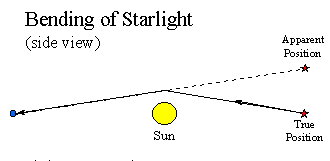
\includegraphics[scale=0.75]{bend.png}
\end{figure}
The star's light was bent by the sun's gravitational field. If instead of accounting for the bend, you looked straight along the line
of light, the star appeared to be in a different position.
\section{Curved Spacetime}
There is another interesting implication of the idea that light is bent by a gravitational field. To understand it, we have to look
at Newton's law of gravity. He said that the gravitational force between two objects is $F=\frac{Gm_1m_2}{r^2}$, where $m_1$ is 
the mass of the first object, $m_2$ is the mass of the second object, $r$ is the distance between the two masses, and $G$ is a constant.
Now, let's say we are looking at how light is curved by the sun. The mass of the sun is a whopping $1.989 \times 10^30$ kilograms. 
Light is made up of photons, which have a mass of...zero kilograms. Can you see the problem here? The whole equation will come out to
zero, yet we know that the gravitational force is not zero in this case! Newton's law, which was established for hundreds of years, is
wrong. 

So what is the right approach? Well, Einstein said that gravity isn't actually a force, but the result of curved "spacetime". You can 
imagine the three dimensions of space plus a fourth of time being a flat rubber sheet. When a mass, like a bowling ball is placed
on the sheet, the sheet bends. A lighter mass, such as a tennis ball, when placed on the sheet near the bowling ball will roll toward
the bowling ball - kind of like gravity. However, in this case we only have two-dimensional space being warped. A better image
would be something like the image below:
\begin{figure}[H]
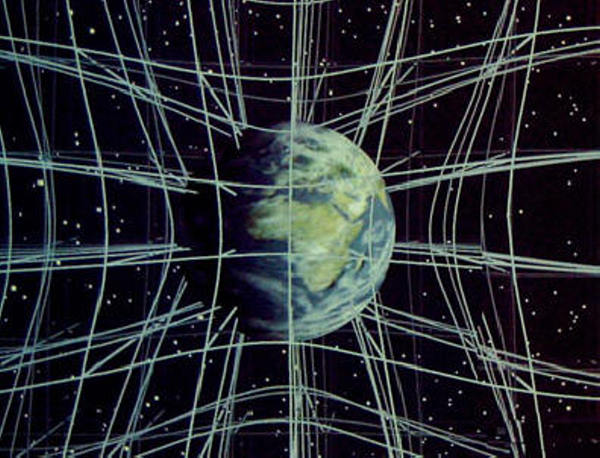
\includegraphics[scale=0.5]{warpspace.jpg}
\end{figure}
However, this still isn't a perfect image, because time isn't warped in this picture, but it's a good enough mental image for now.
So, to summarize, Newton said that gravity was caused by the attraction of two objects, but Einstein said that gravity wasn't
really a thing - objects were just taking the shortest possible path in curved spacetime. 

There is another interesting thing to look at in curved spacetime - spacetime graphs. The first thing to note is the normal three
dimensions of space graphed:
\begin{figure}[H]
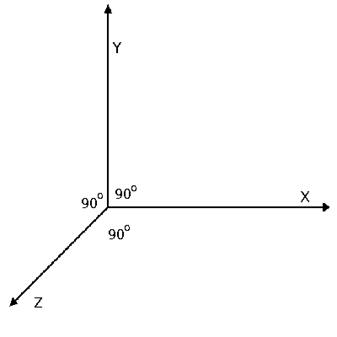
\includegraphics[scale=0.5]{3d.jpg}
\end{figure}
Note that the three axes are at right angles to each other (in math speak, they are orthogonal). If we were to add an axis for the
dimension of time, it would have to be at right angles to all the other axes. Needless to say, this is rather hard to visualize,
so to keep it simple, we're going to stick to one dimension of space and one of time in our graphs. So imagine we have an object 
that is stationary - perhaps your desk, or maybe a book on your shelf. It would be graphed as a straight line up. Why is this? 
Well, the object may not be moving, but time is passing! So there is a straight
line to represent a lack of movement through space, but a steady movement through time. Now, imagine that an object is moving at
a constant velocity. That would look something like this:
\begin{figure}[H]
\includegraphics[scale=0.5]{constanv.jpg}
\end{figure}
It is moving through both space and time, so it is a diagonal line. Another spacetime diagram that is of interest - what would an object
look like that is accelerating?
\begin{figure}[H]
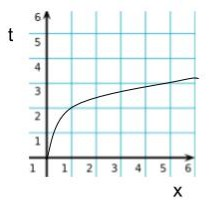
\includegraphics[scale=0.5]{acceler.jpg}
\end{figure}
The line is curved - it is reaching the same location in less time. Finally, it is important to note that the object cannot move
faster than the speed of light. It is common practice to draw the speed of light as 45 degrees from the x-axis, so anything at an
angle less than 45 degrees to the x-axis is expressly forbidden.
\begin{figure}[H]
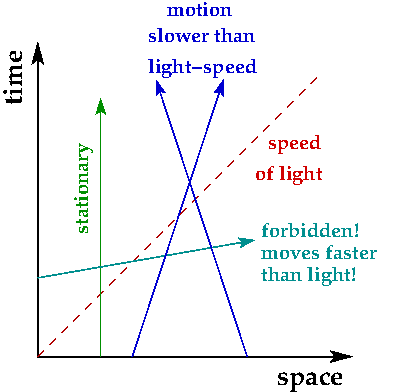
\includegraphics[scale=0.5]{light.png}
\end{figure}
